%
%
\documentclass{cv}

\usepackage[francais]{babel}
\usepackage[utf8]{inputenc}
\usepackage[T1]{fontenc}
\usepackage{graphicx}
\usepackage{hyperref}
\usepackage[svgnames]{xcolor}
\usepackage[paper=a4paper,textwidth=160mm]{geometry}

\newcommand{\lieu}[1]{{#1}\ }
\newcommand{\activite}[1]{\textbf{#1}\ }
\newcommand{\comment}[1]{\textsl{#1}\ }
\usepackage{geometry}
\geometry{ vmargin=1cm, right=1.5cm, left=1.5cm }

\begin{document}

\begin{chapeau}
\begin{adresse}
	Philippe Virouleau\\%
	Bordeaux\\%
	{\color{DarkGreen}{\ligne}}\\%
	Tél. : 06 12 66 62 44\\%
	Mail : \texttt{philippe.44@gmail.com}
\end{adresse}
\begin{titre}
\textbf{Docteur en informatique\\~\\
  Ingénieur Ensimag en Systèmes d'Information}
\end{titre}
\begin{etatcivil}
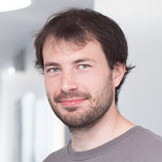
\includegraphics[width=0.7\textwidth]{philippe.png}

	Né le 04/09/1989\\
	Nationalité Française\\
	Permis B
\end{etatcivil}
\end{chapeau}



	%%%%%%%%%%%%%%%%%%
	% Bloc rubriques %
	%%%%%%%%%%%%%%%%%%


\begin{rubriquetableau}[3cm]{Formation}



2015--2018
	& \activite{Docteur en informatique de l'Université Grenoble-Alpes}\\

2009--2012
	& \activite{Ingénieur Ensimag}
	\comment{Obtention du diplôme d'Ingénieur Grenoble INP - Ensimag le 3 Juillet 2012, filière ISI : Ingénierie des Systèmes d'Information}
	\lieu{Grenoble}\\

2007--2009
	& \activite{Classe préparatoire PT}
	\lieu{Lycée Livet, Nantes}\\
Juillet 2007
	& \activite{Baccalauréat Scientifique}
	\comment{Mention Assez Bien}
	\lieu{Lycée Jules Verne, Nantes}\\


\end{rubriquetableau}

\begin{rubrique}{Compétences}%

  \begin{itemize}
    \item Langages maîtrisés : C/C++, Shell, R, Python, Ruby, Javascript

    \item Systèmes d'exploitation : Unix (Debian, Ubuntu), Windows.

    \item Outils et logiciels maîtrisés : Vim, Git/Svn, CMake/Autoconf, outils de débogages usuels (gdb, valgrind, ...), suites bureautiques usuelles.

    \item Compilation : maîtrise du développement au sein de l'infrastructure LLVM/Clang.

    \item Programmation parallèle : maîtrise d'OpenMP, ainsi que des supports exécutifs open source.

      %MPI~: utilisation et développement basique pour des programmes hybrides MPI+OpenMP.

    %\item Connaissances des bibliothèques d'algèbre linéaire BLAS et LAPACK.
    \item Expertise des problématiques liées à l'exploitation des machines à mémoire partagée du type NUMA.
  \end{itemize}

\end{rubrique}


\begin{rubriquetableau}[2.6cm]{Expériences professionnelles}
  Depuis Avr. 2018  & \activite{Post-doctorant au sein des équipes Inria Storm et HiePACS}
    \comment{Exploitation d'architectures hétérogènes (GPUs et systèmes distribués) à l'aide de programmes à base de tâches (OpenMP, StarPU)}
    \lieu{(Inria Bordeaux Sud-Ouest)}\\
Mars 2015 - Mars 2018 & \activite{Doctorant au sein de l'équipe Inria CORSE}
    \comment{Étude et amélioration de l'exploitation des architectures NUMA à travers des supports exécutifs}
    \comment{Thèse impliquant notamment l'évaluation, l'analyse, et l'amélioration d'applications d'algèbre linéaire, ainsi que de nombreux développements au sein de l'infrastructure LLVM/Clang et de supports exécutifs open source, tels que libOMP et xKaapi.}
    \lieu{(Inria Rhône-Alpes)}\\
Oct. 2012 - Fév. 2015
        & \activite{Ingénieur de recherche Inria au sein de l'équipe MOAIS}
  \comment{Contributions au support exécutif de programmation parallèle hétérogène Kaapi. Réalisation d'un compilateur source à source basé sur Clang~: KStar.}
        \lieu{(Inria Rhône-Alpes)}\\

Fév. - Juil. 2012
        & \activite{Stage de fin d'étude chez Sopra Group}
  \comment{Stage en environnement Java EE, réalisation d'une application d'automatisation de tests, basée sur les technologies TestNG et Selenium.}
        \lieu{(Sopra Group, Nantes)}\\
Juil. - Sep. 2011
        & \activite{Stage à la Direction Générale des Finances Publiques}
	\comment{Stage en environnement Java EE, réalisation d'un pool de threads répartissant ses ressources entre ses clients selon différentes stratégies.}
        \lieu{(DGFiP - Tour Bretagne, Nantes)}\\
2009 - 2012
        %& \activite{Projets scolaires}
%\comment{Écriture d'un simulateur MIPS, Mise en place d'un réseau de capteur (programmation d'une couche MAC CSMA/CA et d'un protocole multisaut, Écriture d'un compilateur pour un sous language de java.}
        %\lieu{(Ensimag)}\\
%Mai - Juin 2011
        %& \activite{Projet : Réseau de capteurs}
	%\comment{Projet en binôme, programmation d'une couche MAC de type CSMA/CA et d'un protocole multisaut. Projet en C sur micro-controlleur msp430.}
        %\lieu{(Ensimag)}\\
%2009--2011
        %& \activite{Projet : Compilateur}
	%\comment{Projet en quadrinôme sur un mois, réalisation d'un compilateur pour un sous language de java. Projet réalisé en Ada.}
        %\lieu{(Ensimag)}\\
%~
        %& \activite{Projet : Simulateur MIPS}
	%\comment{Projet en trinôme sur une semaine, réalisation d'un simulateur MIPS en C}
        %\lieu{(Ensimag)}\\
%~
        %& \activite{Moniteur à l'Ensimag}
	%\comment{En charge de la maintenance des serveurs et de la fermeture des salles informatiques de l'Ensimag}
        %\lieu{(Ensimag)}\\
% ~
%         & \activite{Président du Pole Communication de l'Ensimag}
% 	\comment{Administration et organisation de l'association en charge de la communication auprès des élèves de l'Ensimag.}
%         \lieu{(Ensimag, Grenoble)}\\
~
        & \activite{Implication dans la vie associative de l'Ensimag}
	\comment{Président du Pole Communication de l'Ensimag, responsable de la communication externe du Bureau des élèves, ainsi que de l'administration de serveurs apache, svn et git, sous Debian. En charge de la maintenance des serveurs et de la fermeture des salles informatiques de l'Ensimag.}
        \lieu{(Ensimag)}\\
% ~
%         & \activite{Administrateur du serveur du Bureau des élèves de l'Ensimag}
% 	\comment{Administration de serveurs apache, svn et git, sous Debian.}
%         \lieu{(Ensimag, Grenoble)}\\
% ~
%         & \activite{Responsable de la communication externe du Bureau des élèves de l'Ensimag}
% 	\comment{Communication sur les évènements organisés par le bde auprès des élèves, organisation d'évènements de plus de 300 personnes.}
%         \lieu{(Ensimag, Grenoble)}\\
% 2006--2007
% 	& \activite{Portage salarial}
% 	\comment{Conception de sites internet, sauvegarde de VHS et de Vinyles pour des particuliers}
% 	\lieu{(Nantes)}\\
% 2005--2007
% 	& \activite{Membre de l'association humanitaire Sierra Norte}
% 	\comment{Récolte de fonds pour financer la construction d'une école au Mexique, puis d'un dispensaire en Inde après le Tsunami.}
% 	\lieu{(Nantes)}\\
\end{rubriquetableau}

\pagebreak

\begin{rubriquetableau}[3cm]{Publications scientifiques}

Juin 2017
        & \activite{Étude de l'impact d'une clause d'affinité sur les performances et l'énergie dans un support exécutif OpenMP}
	\comment{Philippe Virouleau, Compas 2017}
        \lieu{}\\

Oct. 2016
        & \activite{Description, Implementation and Evaluation of an Affinity Clause for Task Directives}
	\comment{Philippe Virouleau and al., 12th International Workshop on OpenMP, IWOMP2016}
        \lieu{}\\

Août 2016
        & \activite{Using data dependencies to improve task-based scheduling strategies on NUMA architectures}
	\comment{Philippe Virouleau and al., Euro-Par 2016}
        \lieu{}\\

Juillet 2016
        & \activite{Amélioration des stratégies d'ordonnancement sur architectures NUMA à l'aide des dépendances de données}
	\comment{Philippe Virouleau, Compas 2016}
        \lieu{}\\

Oct. 2014
        & \activite{Evaluation of OpenMP Dependent Tasks with the KASTORS Benchmark Suite}
	\comment{Philippe Virouleau and al., 10th International Workshop on OpenMP, IWOMP2014}
        \lieu{}\\
\end{rubriquetableau}

\begin{rubriquetableau}[2.6cm]{Enseignements}
    
2018 - 2019 & \activite{Vacations à l'ENSEIRB-MATMECA}
  \comment{TDs et projets de programmation impérative (C) en 1ère année, TDs et projets de Système d'Exploitation en 2ème année.}
        \\

2012 - 2015 & \activite{Vacations à l'Ensimag}
	\comment{Cours d'Algorithmique et Structures de données en 1ère année, Cours-TD de Système d'Exploitation et Programmation Concurrente en 2ème année.}
        \\
\end{rubriquetableau}


\begin{rubrique}{Langues} 
Anglais, courant.

Espagnol, scolaire.

Russe, notions.
\end{rubrique}




\begin{rubriquetableau}[2.6cm]{Loisirs}
Rubik's Cube 
    & \activite{\href{https://www.worldcubeassociation.org/persons/2008VIRO01}{Pratique en compétition}}
\comment{
  Participation à plus de 100 compétitions (locales et internationales) ayant données lieu à plus de 200 podiums dont 9 titres de champion de France, et 19 records de France.
}
	\\
	& \activite{Organisation et arbitrage de compétitions} 
	\comment{
\begin{itemize}
    \item Arbitre principal au sein de la World Cube Association (WCA) depuis 2010
    \item Président de l'Association Française de Speedcubing de 2014 à 2018.
    \item Membre du comité en charge du règlement des compétitions WCA depuis 2016
    \item Membre de l'équipe logicielle de la WCA depuis 2016
\end{itemize}
Organisation de plusieurs dizaines de compétitions, dont plusieurs championnats de France, d'Europe, et du Monde.
    }
	\\
Ski
	& \activite{Pratique régulière}
	\comment{Pratique depuis l'age de 8 ans}
	\\
\end{rubriquetableau}

\end{document}






